\documentclass{beamer}
\usepackage{geometry}
\usepackage[english]{babel}
\usepackage[utf8]{inputenc}
\usepackage{amsmath}
\usepackage{amsfonts}
\usepackage{amssymb}
\usepackage{tikz}
\usetikzlibrary{quotes, angles}
\usepackage{graphicx}

%\usepackage{pgfplots}
%\pgfplotsset{width=10cm,compat=1.9}
%\usepackage{pgfplotstable}

\usepackage{fancyhdr}
\pagestyle{fancy}
\setlength{\headheight}{12pt}%doesn't seem to fix warning
\fancyhf{}

%\rhead{\small{2 January 2020}}
\lhead{\small{BECA / Dr. Huson / Geometry Unit 8: Area \ volume, solids}}

\renewcommand{\headrulewidth}{0pt}

\title{Mathematics Class Slides}
\subtitle{Bronx Early College Academy}
\author{Chris Huson}
\date{28 January 2020}

\begin{document}
\frame{\titlepage}
\section[Outline]{}
\frame{\tableofcontents}

\section{8.1 Circle and volume formulas, Tuesday 28 January} 
\frame
{
  \frametitle{GQ: How do we calculate the area and circumference of a circle?}
  \framesubtitle{CCSS: HSG.GMD.A1 Circle formulas for circumference and area \hfill \alert{8.1 Tuesday 28 January}}

  \begin{block}{Do Now: Area and volume problems}
  \begin{itemize}
    \item Area of triangles and parallelograms
    \item Volume formula practice
    \item Circle area and circumference
    \item Circle vocabulary
  \end{itemize}
  \end{block}
  Lesson: Circle formulas \& terminology; \\
  Solids formula notation (start with a label variable, $A$, $V$, $C$, $P$)\\*[5pt]
  Homework: Review reference sheets; Deltamath
}

\section{8.2 Estimating, measuring, scale models, Wednesday 29 January}
\frame
{
  \frametitle{GQ: How do we estimate and work with appropriate precision?}
  \framesubtitle{CCSS: HSG.SRT.GMD.A3 Use volume formulas to solve problems \hfill \alert{8.2 Wednesday 29 January}}

  \begin{block}{Do Now: Area and volume problems}
  \begin{itemize}
    \item Circle area and circumference
    \item Volume formula practice
    \item Circle vocabulary
  \end{itemize}
  \end{block}
  Lesson: Scale drawings; Counting squares to estimate area, rounding\\
  Compound shapes\\*[5pt]
  Homework: Khan Academy volume review and introduction to density (watch video)
}

\section{8.3 Density, Thursday 30 January}
\frame
{
  \frametitle{GQ: How do we apply density ratios to calculate weight?}
  \framesubtitle{CCSS: HSG.MG.A2 Apply concepts of density to model \hfill \alert{8.3 Thursday 30 January}}

  \begin{block}{Do Now: Estimating and rounding problems}
  \begin{itemize}
    \item Scale drawing problems
    \item Area and volume formula practice
    \item Solving in terms of $\pi$ and rounding
    \item Compound shapes
  \end{itemize}
  \end{block}
  Lesson: Density ratios, unit changes, cost calculations\\*[5pt]
  Homework: Khan Academy
}

\section{8.4 Equation of a circle, Friday 31 January}
\frame
{
  \frametitle{GQ: How do we define a circle using analytic geometry?}
  \framesubtitle{CCSS: HSG.GPE.A1 Equation of a circle of given center and radius \hfill \alert{8.4 Friday 31 January}}

  \begin{block}{Do Now Quiz: Area and volume problems\\[0.25cm]
    \alert{Classwork counts double while Dr. Huson is out!}}
  \begin{itemize}
    \item Circle vocabulary
    \item Area and volume formula practice
    \item Solving in terms of $\pi$ and rounding
    \item Compound shapes
  \end{itemize}
  \end{block}
  Lesson: Equation of a circle $(x-a)^2+(y-b)^2=r^2$\\*[5pt]
  Homework: Deltamath due Sunday 10:00pm
}

\section{8.5 Cross sections in 3-dimensions, Monday 3 February}
\frame
{
  \frametitle{GQ: How do we imagine objects 3-dimensions?}
  \framesubtitle{CCSS: HSG.SRT.GMD.A3 Use volume formulas to solve problems \hfill \alert{8.5 Monday 3 February}}

  \begin{block}{Do Now: Area and volume problems\\[0.25cm]
    \alert{Classwork counts double while Dr. Huson is out!}}
  \begin{itemize}
    \item Circle and sector areas
    \item Area and volume formula practice
    \item Equation of a circle
  \end{itemize}
  \end{block}
  Lesson: Cross sections in 3-dimensions\\*[5pt]
  Homework: Complete solids and cross sections handout.
}

\section{8.6 Rotations in 3-dimensions, Cross sections, Tuesday 4 February}
\frame
{
  \frametitle{GQ: How do we imagine a figure rotated in space?}
  \framesubtitle{CCSS: HSG.SRT.GMD.A3 Use volume formulas to solve problems \hfill \alert{8.6 Tuesday 4 February}}

  \begin{block}{Do Now: Circle problems}
  \begin{itemize}
    \item Circle equations, the distance formula
    \item Area and volume formula practice
    \item Volume and density application
  \end{itemize}
  \end{block}
  Lesson: Rotations in 3-dimensions, Cross sections\\*[5pt]
  Homework: Handout area, volume, and density problems
}

\section{8.7 Review for unit test, Wednesday 5 February}
\frame
{
  \frametitle{GQ: How do we calculate area and volume?}
  \framesubtitle{CCSS: HSG.SRT.GMD.A3 Use volume formulas to solve problems \hfill \alert{8.7 Wednesday 5 February}}

  \begin{block}{Do Now: Circle problems}
  \begin{itemize}
    \item Algebra practice
    \item Area and volume formula practice
    \item Volume and density application
  \end{itemize}
  \end{block}
  Lesson: Review for unit exam\\*[5pt]
  Homework: Handout review problems, study for \alert{Test Tomorrow}
}

\section{8.8 Exam: areas, circles, volumes, Thursday 6 February}
\frame
{
  \frametitle{GQ: How do we calculate area and volume?}
  \framesubtitle{CCSS: HSG.SRT.GMD.A3 Use volume formulas to solve problems \hfill \alert{8.8 Thursday 6 February}}

  \begin{block}{Unit test: Area \& volume}
  \begin{itemize}
    \item Circle terminology, sectors
    \item Area and volume formulas
    \item Volume and density applications
  \end{itemize}
  \end{block}
  Homework: Deltamath due 10:00pm
}

\section{8.9 Calculator circle equations, Friday 7 February}
\frame
{
  \frametitle{GQ: How do we define a circle with an equation?}
  \framesubtitle{CCSS: HSG.GPE.A1 Equation of a circle of given center and radius \hfill \alert{8.9 Friday 7 February}}

  \begin{block}{Do Now: Circle problems}
  \begin{itemize}
    \item Circle equations, the distance formula
    \item Algebra practice
  \end{itemize}
  \end{block}
  Lesson: Calculator graphing equation of a circle $(x-a)^2+(y-b)^2=r^2 \rightarrow x^2-2ax+y^2-2by=r^2-a^2-b^2$\\[5pt]
  Homework: Deltamath due 10:00pm Sunday
}

\section{8.10 Calculator circle equations, Monday 10 February}
\frame
{
  \frametitle{GQ: How do we define a circle with an equation?}
  \framesubtitle{CCSS: HSG.GPE.A1 Equation of a circle of given center and radius \hfill \alert{8.10 Monday 10 February}}

  \begin{block}{Do Now: Find the circle center and radius using a calculator}
  \begin{enumerate}
    \item $x^2-6x+y^2+10y = -18$
    \item $x^2+y^2+14x-2y = 14$
  \end{enumerate}
  \end{block}
  Lesson: Compound solid shapes\\[5pt]
  Homework: Deltamath due 10:00pm Tuesday
}

\section{8.11 Compound volume situations, Wednesday 12 February}
\frame
{
  \frametitle{GQ: How do we combine solids?}
  \framesubtitle{CCSS: HSG.GPE.A1 Equation of a circle of given center and radius \hfill \alert{8.11 Wednesday 12 February}}

  \begin{block}{Do Now: Circle problems}
  \begin{itemize}
    \item Circle equations, the distance formula
    \item Algebra practice
  \end{itemize}
  \end{block}
  Lesson: Water tank volume problems\\[5pt]
  Homework: Deltamath due 10:00pm
}

\section{8.11 Compound volume situations, Wednesday 12 February}
\frame
{
  \frametitle{Do Now: Combine the areas of figures}
  \framesubtitle{CCSS: HSG.GPE.A1 Equation of a circle of given center, radius \hfill \alert{8.11 Wednesday 12 Feb}}

  \begin{itemize}
    \item Copy definition: \alert{slant height} - the diagonal length of a triangle, cone, or pyramid
    \item Find the area of the figure (triangle+rectangle+semi-circle)
  \end{itemize}
  \begin{flushright}
    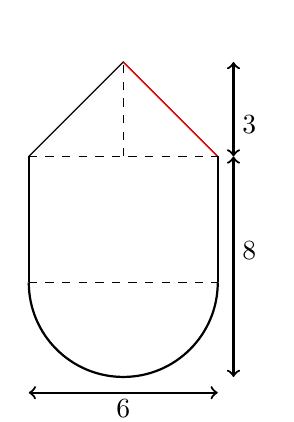
\begin{tikzpicture}[scale=.4]
      %\draw [help lines] (-2,-4) grid (8,12);
      %\draw [thick, ->] (-2.2,0) -- (8.4,0) node [below right] {$x$};
      %\draw [thick, ->] (0,-1.2)--(0,7.4) node [left] {$y$};
      \draw [thick] (0,0)--(0,4);
      \draw [thick] (6,0)--(6,4);
      \draw [] (0,4)--(3,7)--(6,4);
      \draw [red] (3,7)--(6,4);
      \draw [thick] (0,0) arc (180:360:3);
      %\draw [thick] (0,0) arc (-110:-70:8.9);
      \draw [dashed] (0,0) --(6,0);
      \draw [dashed] (0,4) --(6,4);
      \draw [dashed] (3,4) --(3,7);
      %\draw [thick] (0,8) arc (-110:-70:8.9);
      %\draw [dashed] (0,8) arc (110:70:8.9);
      \draw [thick, <->] (6.5,-3)--(6.5,4);
      \node at (7,1){$8$};
      \draw [thick, <->] (6.5,4)--(6.5,7);
      \node at (7,5){$3$};
      \draw [thick, <->] (0,-3.5)--(6,-3.5);
      \node at (3,-4){$6$};
    \end{tikzpicture}
  \end{flushright}
}

\section{8.12 Compound volume situations, Thursday 13 February}
\frame
{
  \frametitle{GQ: How do we combine solids?}
  \framesubtitle{CCSS: HSG.GPE.A1 Equation of a circle of given center and radius \hfill \alert{8.12 Thursday 13 February}}

  \begin{block}{Do Now: Circle problems}
  \begin{itemize}
    \item Circle and sector problems, the distance formula
    \item Volume and area formula practice
  \end{itemize}
  \end{block}
  Lesson: Volume problems\\[5pt]
  Homework: Deltamath due 10:00pm
}

\section{8.13 Compound volume situations, Friday 14 February}
\frame
{
  \frametitle{GQ: How do we combine solids?}
  \framesubtitle{CCSS: HSG.GPE.A1 Equation of a circle of given center and radius \hfill \alert{8.13 Friday 14 February}}

  \begin{block}{Do Now: Circle problems}
  \begin{itemize}
    \item Circle and sector problems, the distance formula
    \item Volume and area formula practice
  \end{itemize}
  \end{block}
  Lesson: Volume problems\\[5pt]
  Homework: Enjoy your break!
}

\end{document}

